\section{Compilar e instalar nginx}

\subsection{Preparando el entorno}
Usaremos los pasos indicados en \cite{nginx_baul}, lo primero que debemos
hacer es instalar las dependencias necesarias para la compilación, para ello:
\begin{bashcode}
apt-get install build-essential libssl-dev libpcre3-dev
\end{bashcode}
Tras esto descargamos la última versión de nginx, al momento de escribir
este texto la 1.4.4:
\begin{bashcode}
wget http://nginx.org/download/nginx-1.4.4.tar.gz
\end{bashcode}
Descomprimimos el archivo:
\begin{bashcode}
tar xzvf nginx-1.4.4.tar.gz
\end{bashcode}
Antes de compilar cambiaremos un valor en el código fuente como medida
de seguridad por ocultación. El valor a cambiar es la cadena asignada
a la cabecera que indica el servidor usado en las peticiones HTTP. En
concreto el archivo a cambiar es el alojado en \verb!src/http/ngx_http_header_filter_module.c!,
concretamente en la línea 48:
\begin{ccode}
static char ngx_http_server_string[] = "Server: nginx" CRLF;
static char ngx_http_server_full_string[] = "Server: " NGINX_VER CRLF;
\end{ccode}
Cambiamos estas dos líneas a algo del estilo:
\begin{ccode}
static char ngx_http_server_string[] = "Server: Mi servidor Web" CRLF;
static char ngx_http_server_full_string[] = "Server: Mi servidor Web" CRLF;
\end{ccode}
Ya solo queda compilarlo e instalarlo, de momento necesitaremos los módulos siguientes:
\begin{bashcode}
--with-http_gzip_static_module --sbin-path=/usr/local/sbin
-with-http_ssl_module --without-mail_pop3_module --without-mail_imap_module
--without-mail_smtp_module --with-http_stub_status_module --with-http_realip_module
\end{bashcode}
Aquí estamos habilitando la compresión de las páginas con gzip, SSL para conexiones
seguras, deshabilitando el módulo de correo POP3, IMAP  y SMTP.

Dependiendo de las necesidades de nuestro servidor, deberemos activar o
desactivar algunos módulos. Más tarde necesitaremos recompilar para añadir
el módulo \verb!pagespeed!. La lista de todos los módulos disponibles
se puede consultar en \cite{modules}

\subsection{Compilar}

Ya está todo listo para compilar e instalar, dentro del directorio de
nginx ejecutamos:
\begin{bashcode}
./configure --with-http_gzip_static_module --sbin-path=/usr/local/sbin \
--with-http_ssl_module --without-mail_pop3_module --without-mail_imap_module\
--without-mail_smtp_module --with-http_stub_status_module --with-http_realip_module
\end{bashcode}
Tras esto deberíamos ver un resumen de la operación realizada:
\begin{bashcode}
Configuration summary
  + using system PCRE library
  + using system OpenSSL library
  + md5: using OpenSSL library
  + sha1: using OpenSSL library
  + using system zlib library

  nginx path prefix: "/usr/local/nginx"
  nginx binary file: "/usr/local/sbin"
  nginx configuration prefix: "/usr/local/nginx/conf"
  nginx configuration file: "/usr/local/nginx/conf/nginx.conf"
  nginx pid file: "/usr/local/nginx/logs/nginx.pid"
  nginx error log file: "/usr/local/nginx/logs/error.log"
  nginx http access log file: "/usr/local/nginx/logs/access.log"
  nginx http client request body temporary files: "client_body_temp"
  nginx http proxy temporary files: "proxy_temp"
  nginx http fastcgi temporary files: "fastcgi_temp"
  nginx http uwsgi temporary files: "uwsgi_temp"
  nginx http scgi temporary files: "scgi_temp"
\end{bashcode}
Para compilar e instalar:
\begin{bashcode}
make -j 4 && make install
\end{bashcode}
Tras esto, es necesario descargar el script que permite iniciar, detener,
reiniciar y recargar nginx mediante el comando \verb!service!, podemos descargarlo
desde
\begin{bashcode}
wget https://raw.github.com/JasonGiedymin/nginx-init-ubuntu/master/nginx
mv nginx /etc/init.d/nginx
sudo chmod +x /etc/init.d/nginx
sudo chown root:root /etc/init.d/nginx
update-rc.d nginx defaults
\end{bashcode}
Con esto hemos descargaro el script, lo hemos movido al directorio en el que será
llamado al inicio del sistema, dado permisos de ejecución y asignado a root como
propietario. Hecho esto, para iniciar nuestro servidor web hay que ejecutar
el comando:
\begin{bashcode}
service nginx start
\end{bashcode}
Como se muestra en la figura~\ref{nginx1}, podemos comprobar que nginx está
funcionando correctamente dirigiéndonos a la dirección \verb!localhost!,
donde veremos lo siguiente:
\begin{figure}[H]
\centering
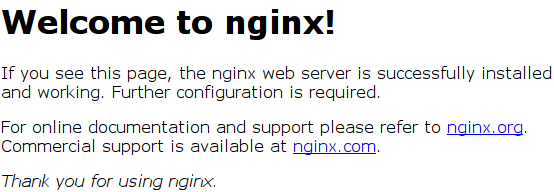
\includegraphics[scale=.5]{./img/instalacionNginx.png}
\caption{Nginx recién instalado}
\label{nginx1}
\end{figure}

En la figura~\ref{serverheader} podemos comprobar la modificación que
hicimos en el código fuente y ver cómo se está ocultando la versión y
tipo de servidor usado:
\begin{figure}[H]
\centering
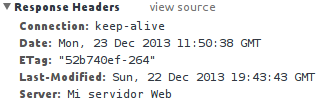
\includegraphics[scale=.5]{./img/serverHeader.png}
\caption{Comprobando la cabecera HTTP Server:}
\label{serverheader}
\end{figure}

\subsection{Configuración}

Ya que está todo listo, vamos a realizar unos cuantos ajustes a la configuración
por defecto:

\begin{bashcode}
user  www-data;
worker_processes  1;

pid        /var/run/nginx.pid;

error_log  logs/error.log;

events {
    worker_connections  1024;
}

http {
    include       mime.types;
    default_type  application/octet-stream;

    gzip on;
    gzip_buffers 16 8k;
    gzip_disable "MSIE [1-6]\.";
    gzip_proxied any;
    gzip_types text/plain text/css application/json application/x-javascript\
               text/xml application/xml application/xml+rss text/javascript;

    log_format  main  '$remote_addr - $remote_user [$time_local] "$request" '
                      '$status $body_bytes_sent "$http_referer" '
                      '"$http_user_agent" "$http_x_forwarded_for"';

    access_log  logs/access.log  main;

    sendfile        on;
    keepalive_timeout  3;
    index              index.html index.htm;

    server {
        listen       80;
        server_name localhost;
        root html;

    access_log  logs/host.access.log  main;

        # Deny all attempts to access hidden files such as .htaccess, .htpasswd, .DS_Store (Mac).
        location ~ /\. {
                deny all;
                access_log off;
                log_not_found off;
        }

    }

}
\end{bashcode}

Los cambios más relevantes sobre la configuración por defecto son:
\begin{itemize}
    \item Se ha cambiado el usuario del servidor de \textit{nobody} a \textit{www-data},
        éste último es el usuario por defecto para servidores webs.
    \item Se define el archivo donde se localizará el PID (Process ID) del
        servidor. Esto permite al script que hemos instalado iniciar o detener nginx.
    \item Se habilita la compresión gzip para reducir el ancho de banda consumido.
    \item Se define el formato que tendrán los ficheros de log.
\end{itemize}

Cambiamos los permisos del directorio donde se alojan los recursos web a
este último usuario y reiniciamos nginx:

\begin{bashcode}
chown -R www-data:www-data /usr/local/nginx/html/
service nginx destroy && service nginx start
\end{bashcode}
